\documentclass[final,hyperref={pdfpagelabels=false},aspectratio=169,t]{beamer}
\mode<presentation> {
  \usecolortheme{rose}
  \setbeamertemplate{footline}[page number] 
  \setbeamertemplate{navigation symbols}{} 
  \usefonttheme{professionalfonts}}


\usepackage{graphicx} % Allows including images
\usepackage{booktabs} % Allows the use of \toprule, \midrule and \bottomrule in tables

\usepackage{geometry}
\usepackage{xspace}

\usepackage[utf8]{inputenc}
\usepackage{default}
\usepackage{amsmath}
\usepackage{amsfonts}
\usepackage{amssymb}
\usepackage{amsthm}
\usepackage{bm}
\usepackage{slashed}

\usepackage{tikz}

\usepackage[overlay,absolute]{textpos}
\setlength{\TPHorizModule}{1cm}
\setlength{\TPVertModule}{1cm}
\textblockorigin{10mm}{10mm}
\input{/Users/marin/tex/GA/presentations/NewCommands.tex}

\graphicspath{
  {./IMAGES/}
{/Users/marin/tex/GA/presentations/}
{/Users/marin/PhysicsTalks/PhysicsFigures/}
}


%----------------------------------------------------------------------------------------
%       TITLE PAGE
%----------------------------------------------------------------------------------------

\date{\today} % Date, can be changed to a custom date

\title{\texorpdfstring{\LARGE Photon Conversion Method for ALICE 3.  \\ $\chi_{\rm C}$ reconstruction. }}
%N$^\gamma$/N$_{ch}$\\ 
%Study of Inclusive photons in RBins 

\author[A.Marin]{Ana Marin}
\institute[GSI]{\small GSI, Darmstadt, Germany}
%\today
\author[GSI]{A.~Marin \inst{1}, A. Uras \inst{2}}
%\author[Hei]{ K. Reygers, J. Stachel}
\institute[GSI]{\inst{1} GSI, Darmstadt, Germany ,  \inst{2} Centre National de la Recherche Scientifique, Lyon, France }

\begin{document}
\begin{frame}

  \begin{textblock}{14}(0.0,1.0)
    \titlepage
  \end{textblock}
  

 % the logos
 \begin{textblock}{12}(0.0,5.7)
     \includegraphics[width=3cm]{GSI_Logo_cmyk}
\end{textblock}

  \begin{textblock}{12}(11.,5.2)
    \includegraphics[width=1.5cm]{2012-Jul-04-4_Color_Logo_CB}
  \end{textblock}

\end{frame}

%-----------------------------------------------
\begin{frame}
\frametitle{Simulation  and reconstruction settings}

\begin{itemize}
\item  Full simulations of pp $\sqrt{s} =$ 14 TeV using PYTHIA 8.2  in local HD cluster  (2.2$\times$10$^6$events generated) 
\item  Analysis using MC information: \\
 Central: $|\eta| < $1.3 (\pT $ > $ 0.1 \GeVc) \\
 Forward: 1.75$ < |\eta| < $ 4 (p $ > $ 0.1 \GeVc)   
 \item Conversion vertices:  (5 layers for reconstruction )\\
 Central: maxR = 22 cm\\
 Forward: -135 $<$  Z  $<$ 135 cm
 
 
\end{itemize}
\end{frame}

%-------------------------------------------

\begin{frame}
\frametitle{Photon Conversion vertices}

\centering
\includegraphics[width=0.48\textwidth]{/Users/marin/alice3/chic/plots/rVSz.png}
\includegraphics[width=0.48\textwidth]{/Users/marin/alice3/alice3Conversions/anaConv/rVSzConvForwardNew.png}


\end{frame}

%------------------------------------------------

\begin{frame}
\frametitle{Central Barrel: $\gamma$ reconstruction} 
%\vspace{1cm}
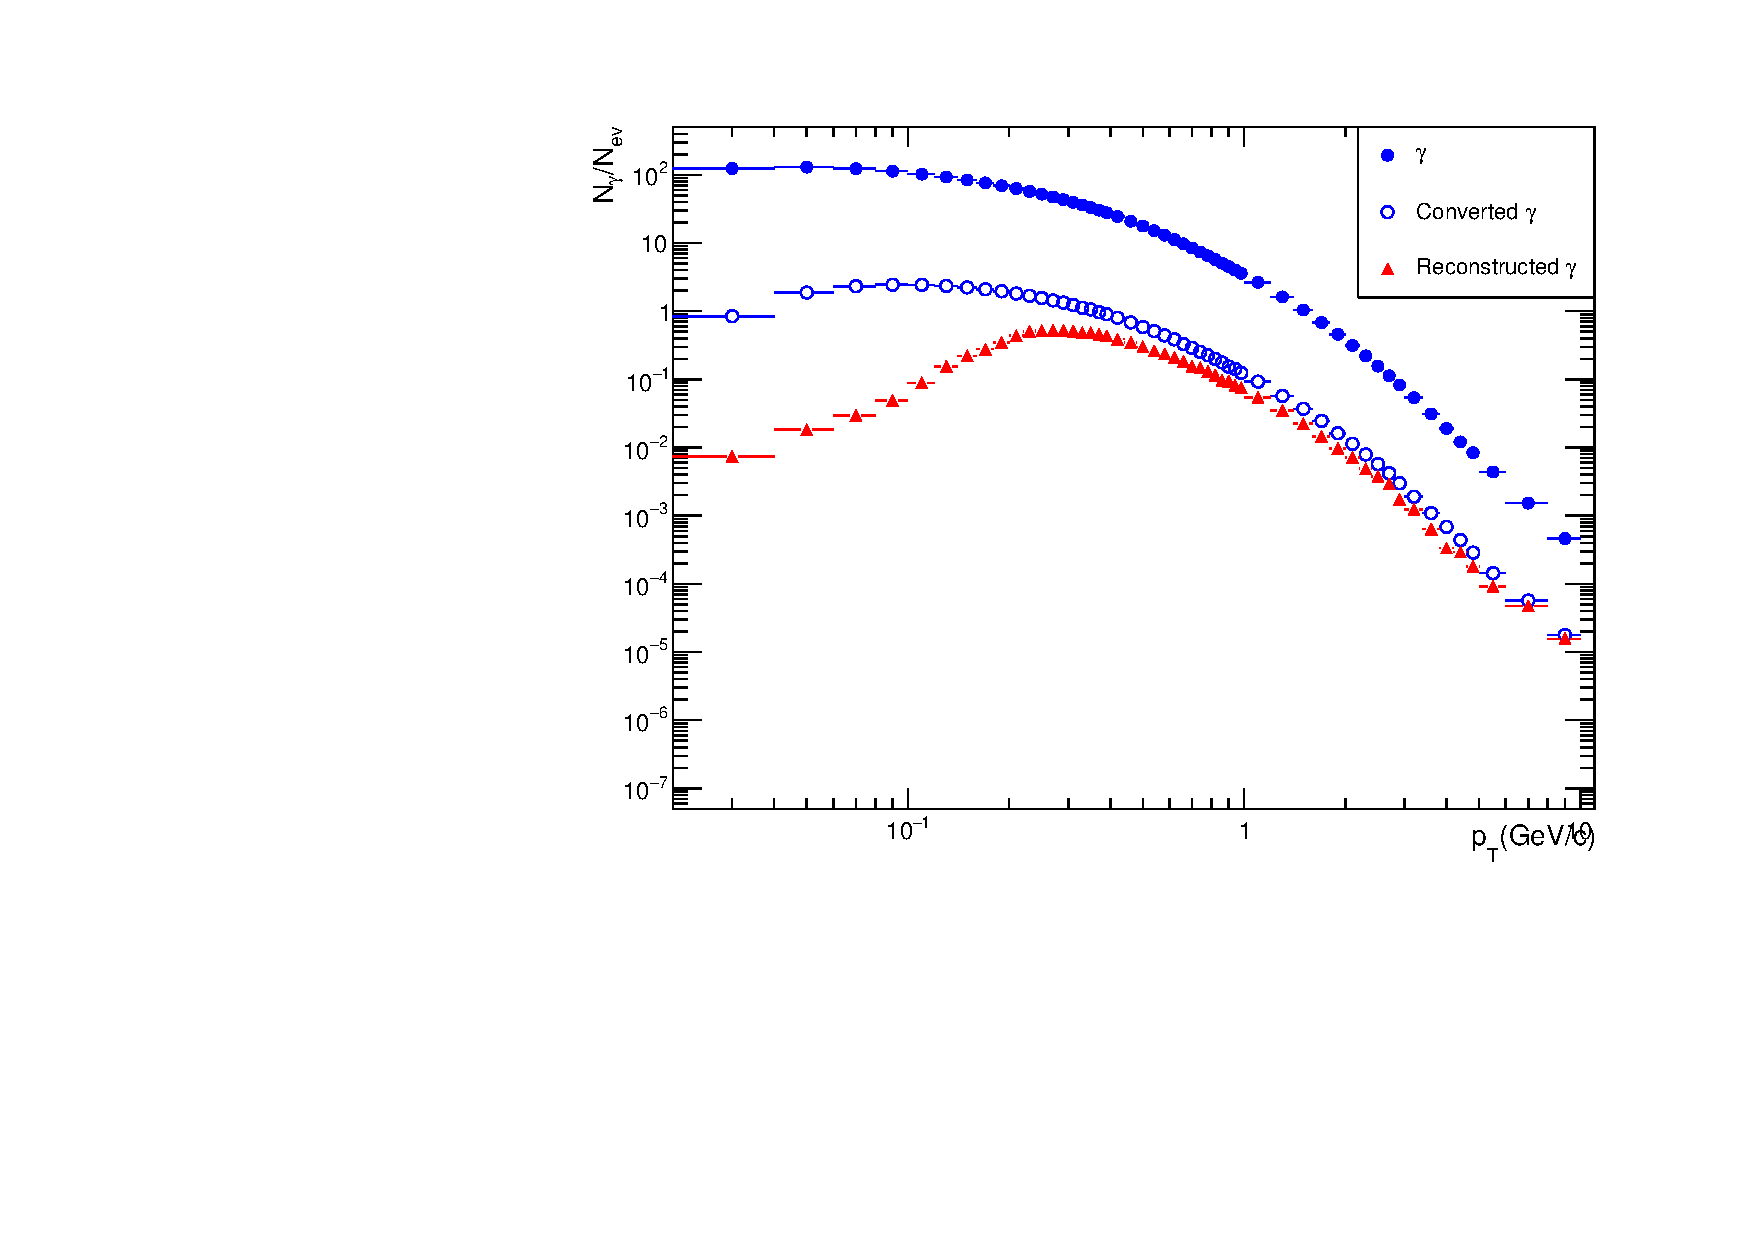
\includegraphics[width=0.38\textwidth]{/Users/marin/alice3/alice3Conversions/anaConv/files220103/PhotonPrimConvRec.pdf}
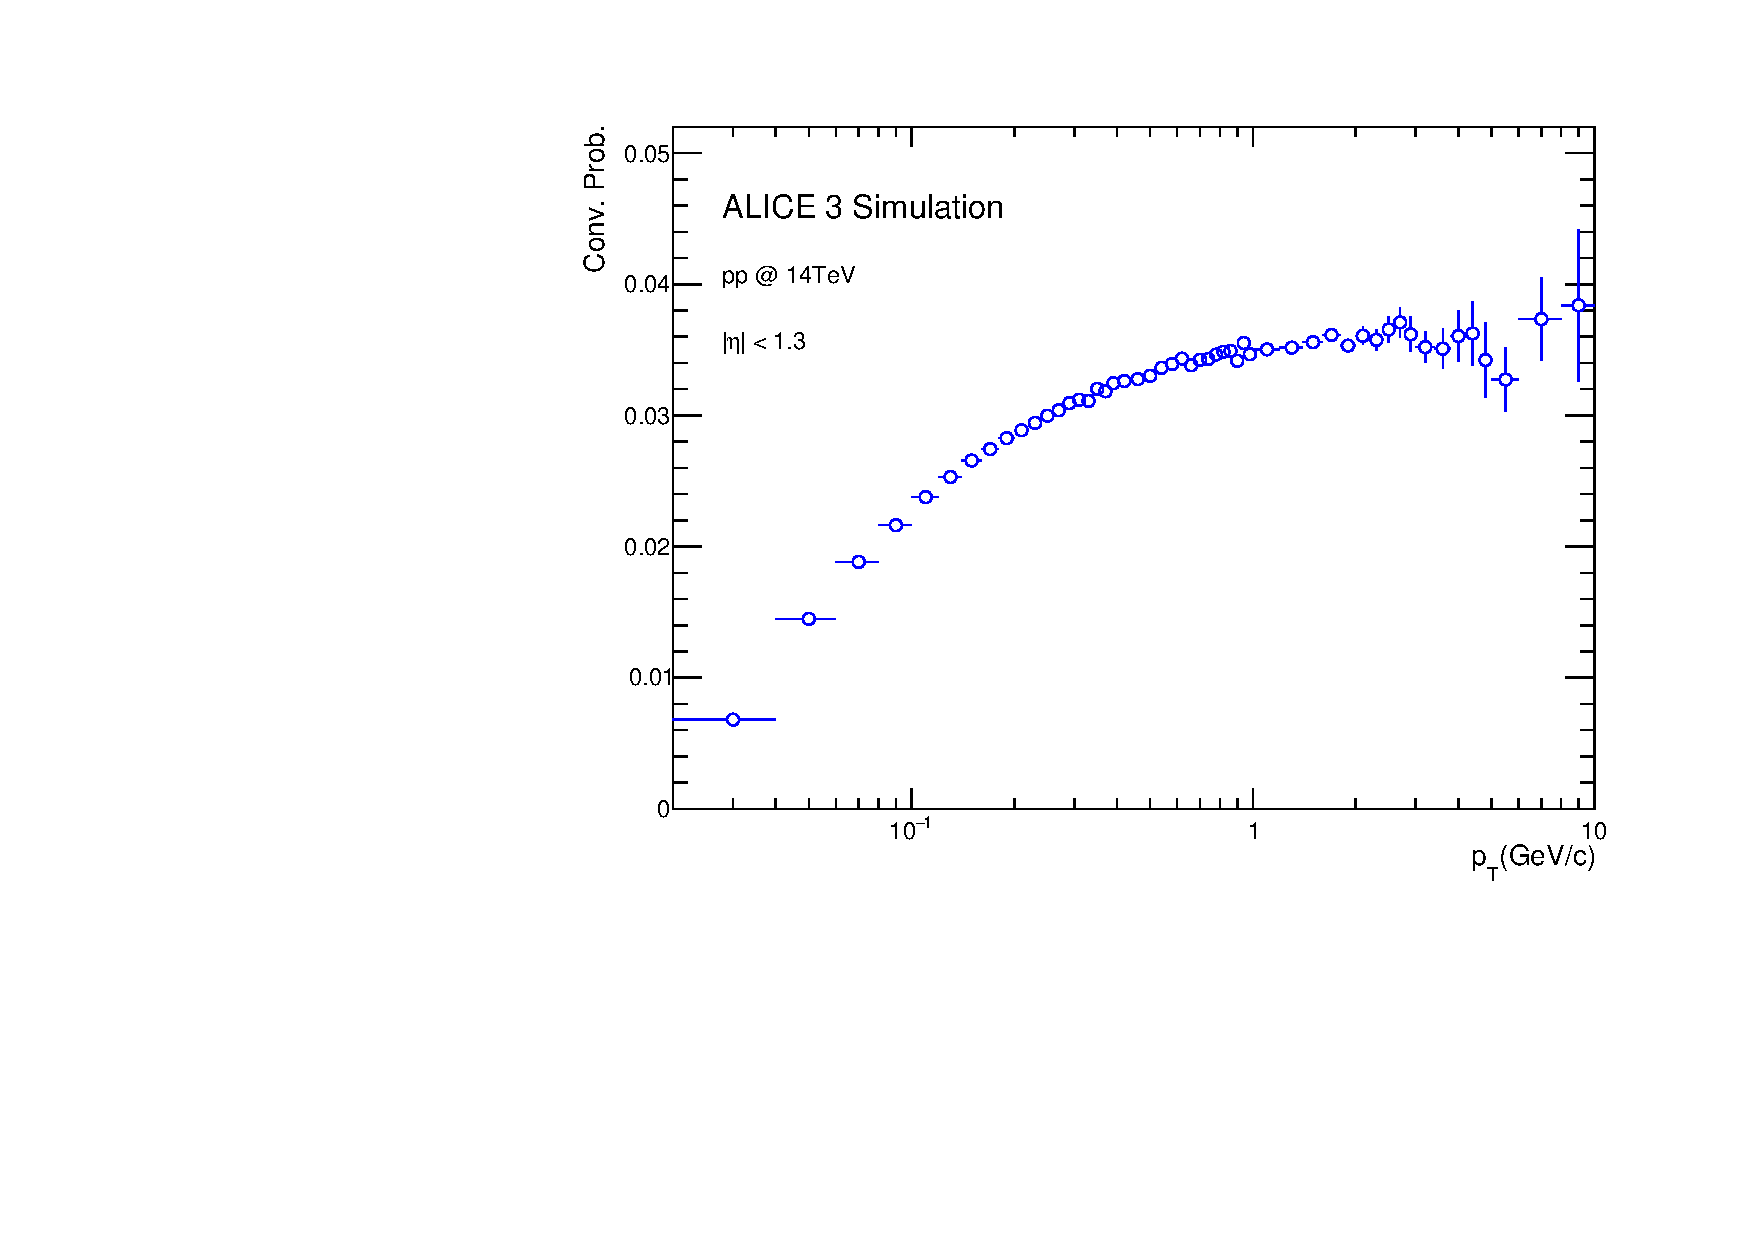
\includegraphics[width=0.38\textwidth]{/Users/marin/alice3/alice3Conversions/anaConv/files220103/PhotonConvProb.pdf}
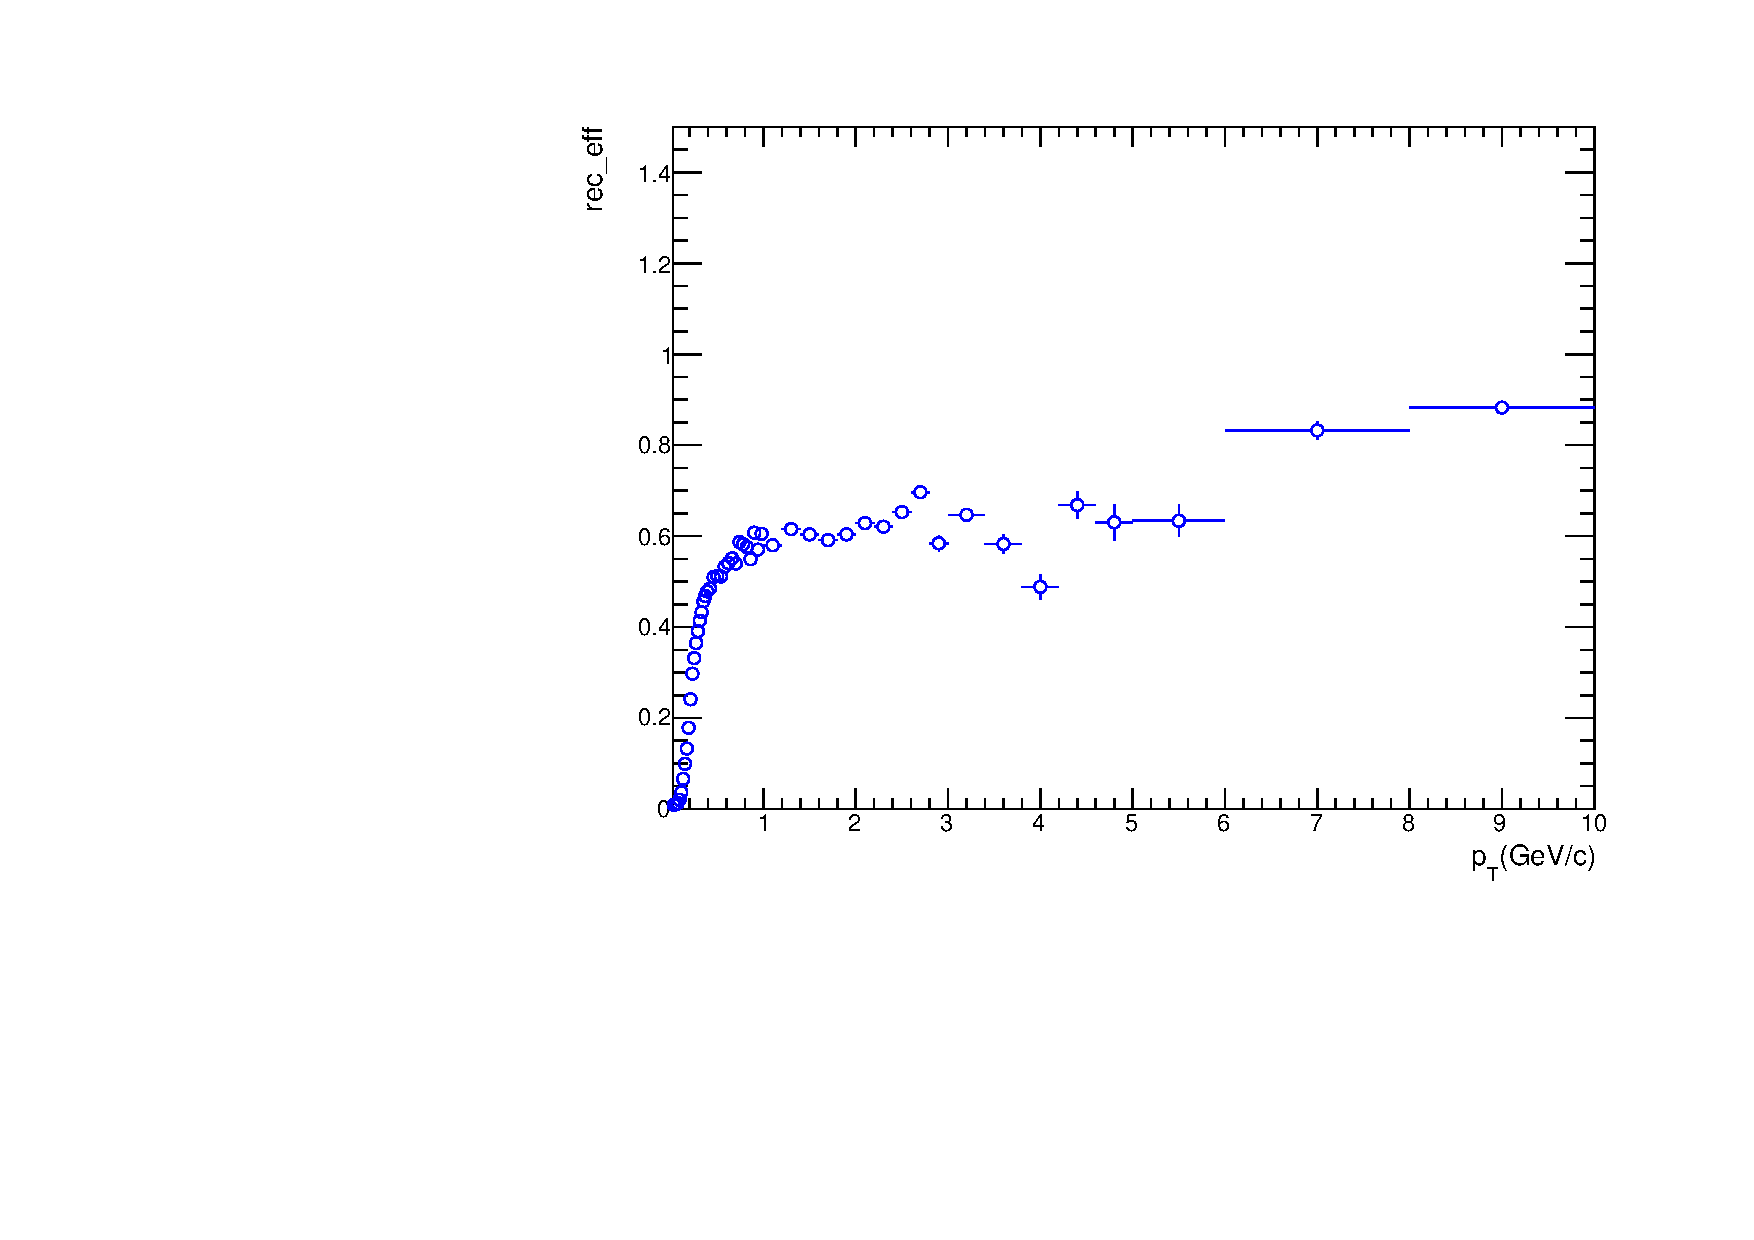
\includegraphics[width=0.38\textwidth]{/Users/marin/alice3/alice3Conversions/anaConv/files220103/PhotonRecEff.pdf}
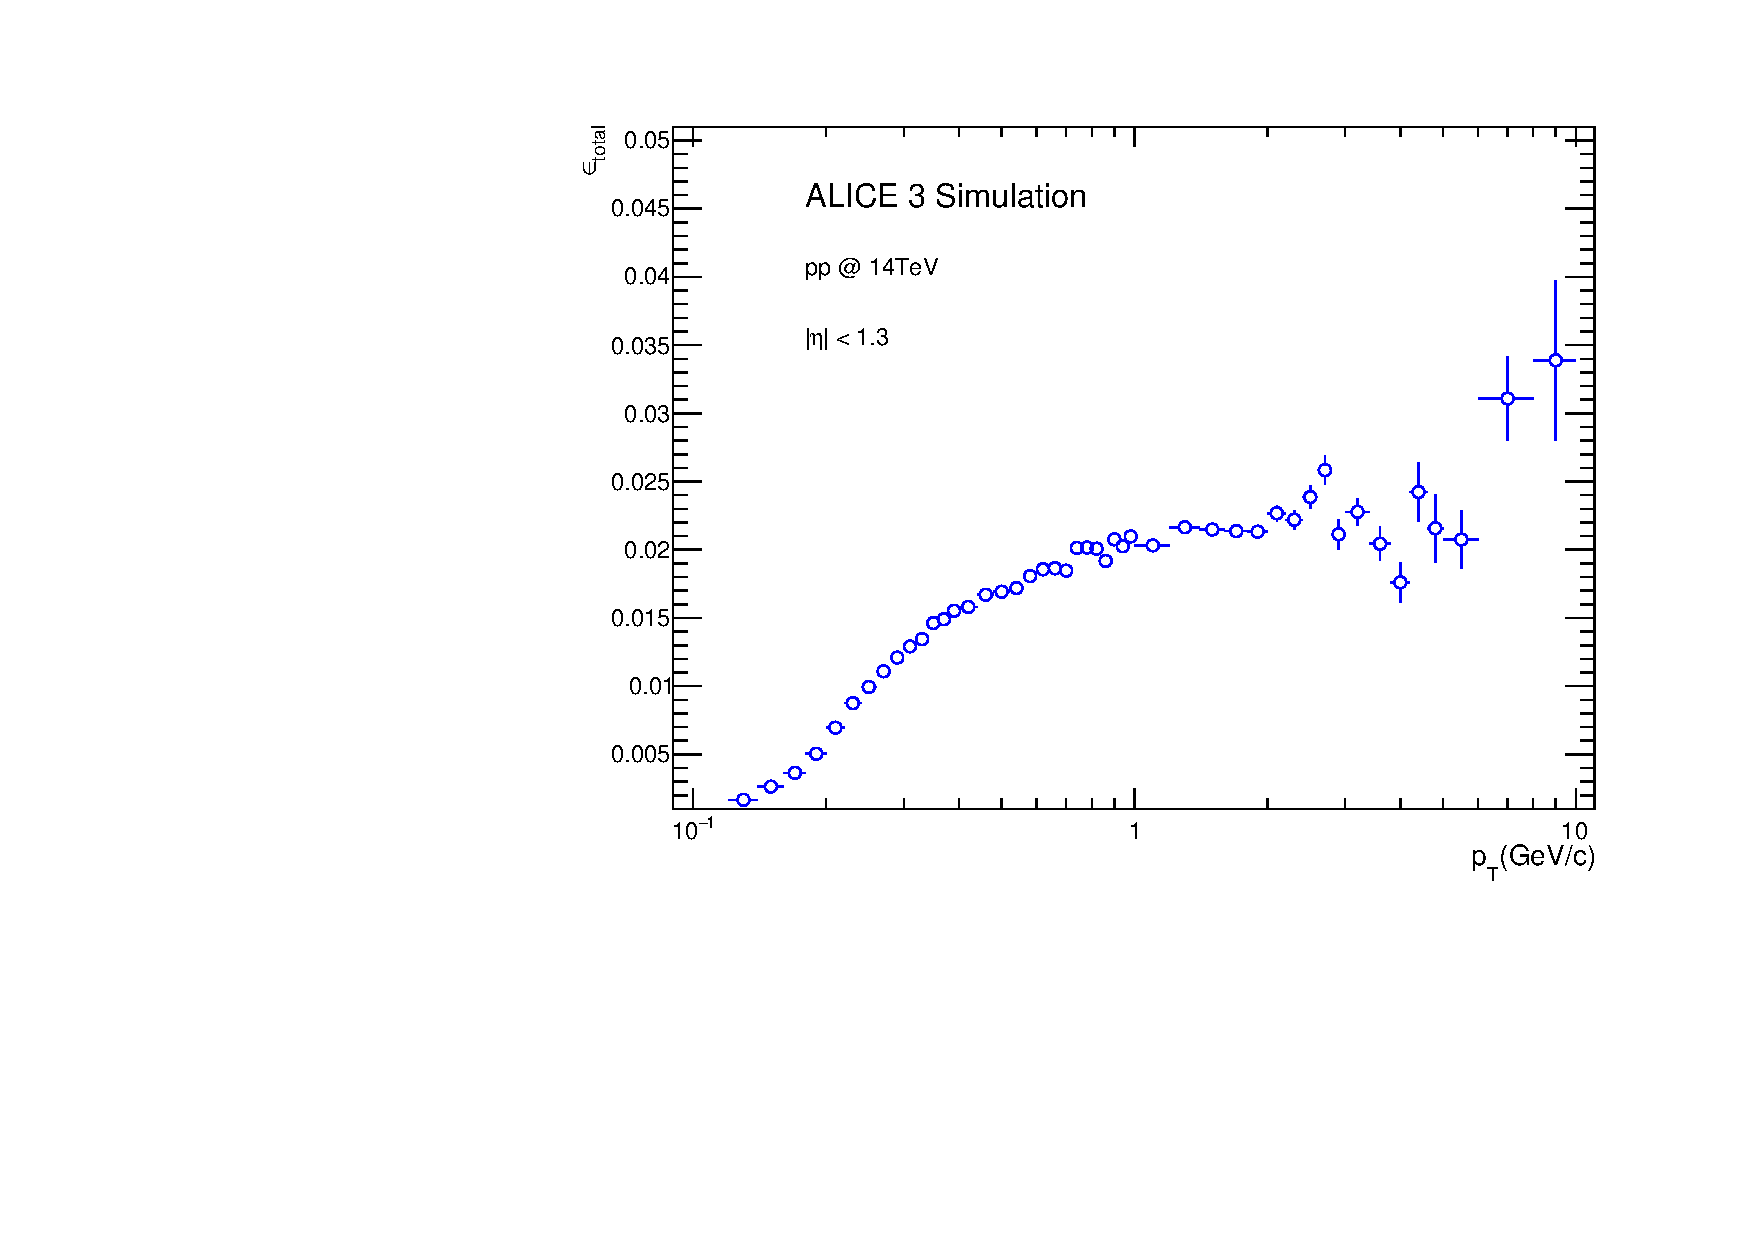
\includegraphics[width=0.38\textwidth]{/Users/marin/alice3/alice3Conversions/anaConv/files220103/totEff.pdf}
\end{frame}

\begin{frame}
\frametitle{Central Barrel: $\gamma$ resolution} 

%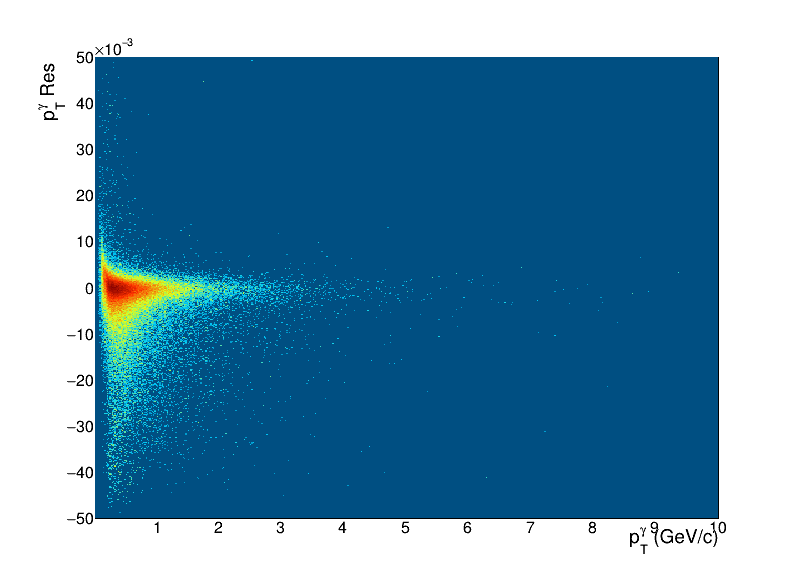
\includegraphics[width=0.38\textwidth]{/Users/marin/alice3/alice3Conversions/anaConv/files220103/PhotonRes.png}

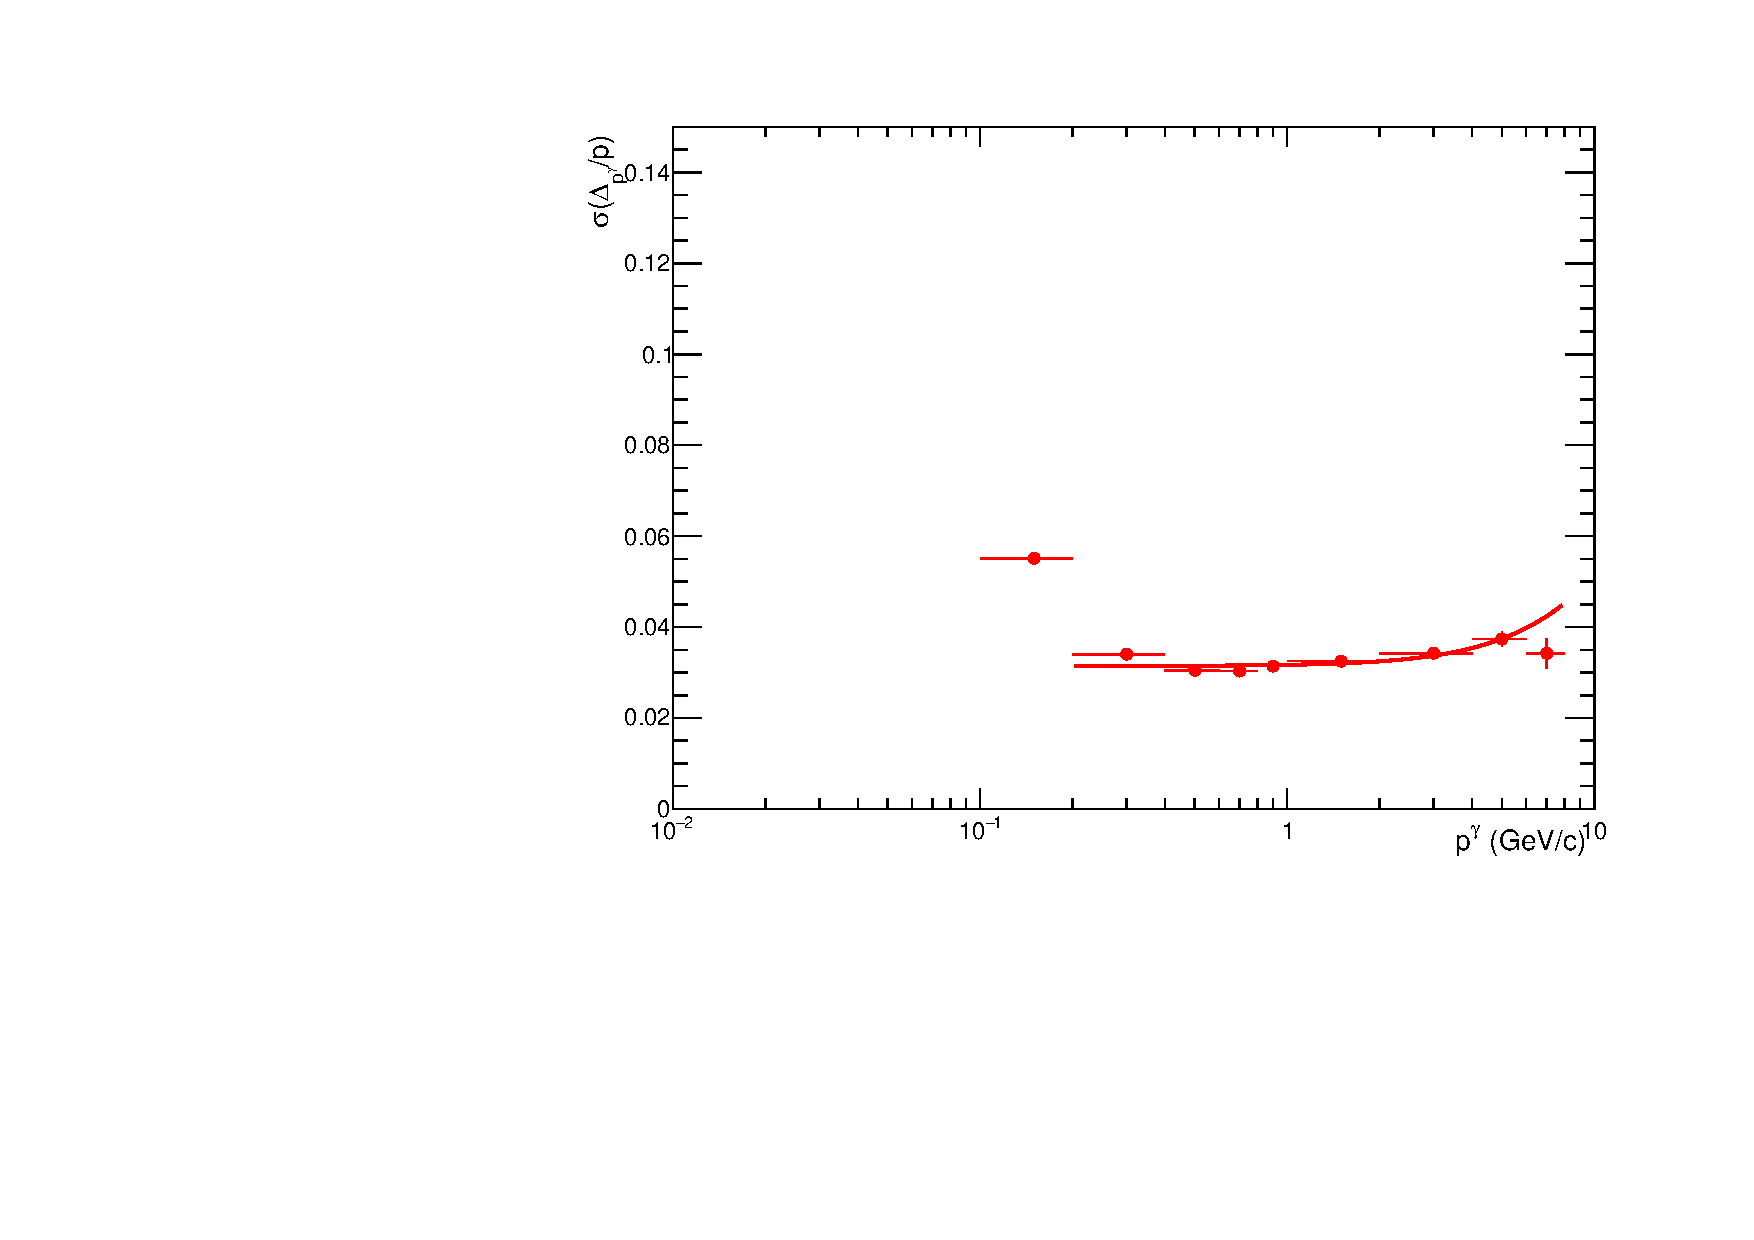
\includegraphics[width=0.38\textwidth]{/Users/marin/alice3/alice3Conversions/anaConv/files220103/PhotonResSigma.pdf}
\end{frame}

\begin{frame}
\frametitle{Forward Barrel: $\gamma$ reconstruction} 

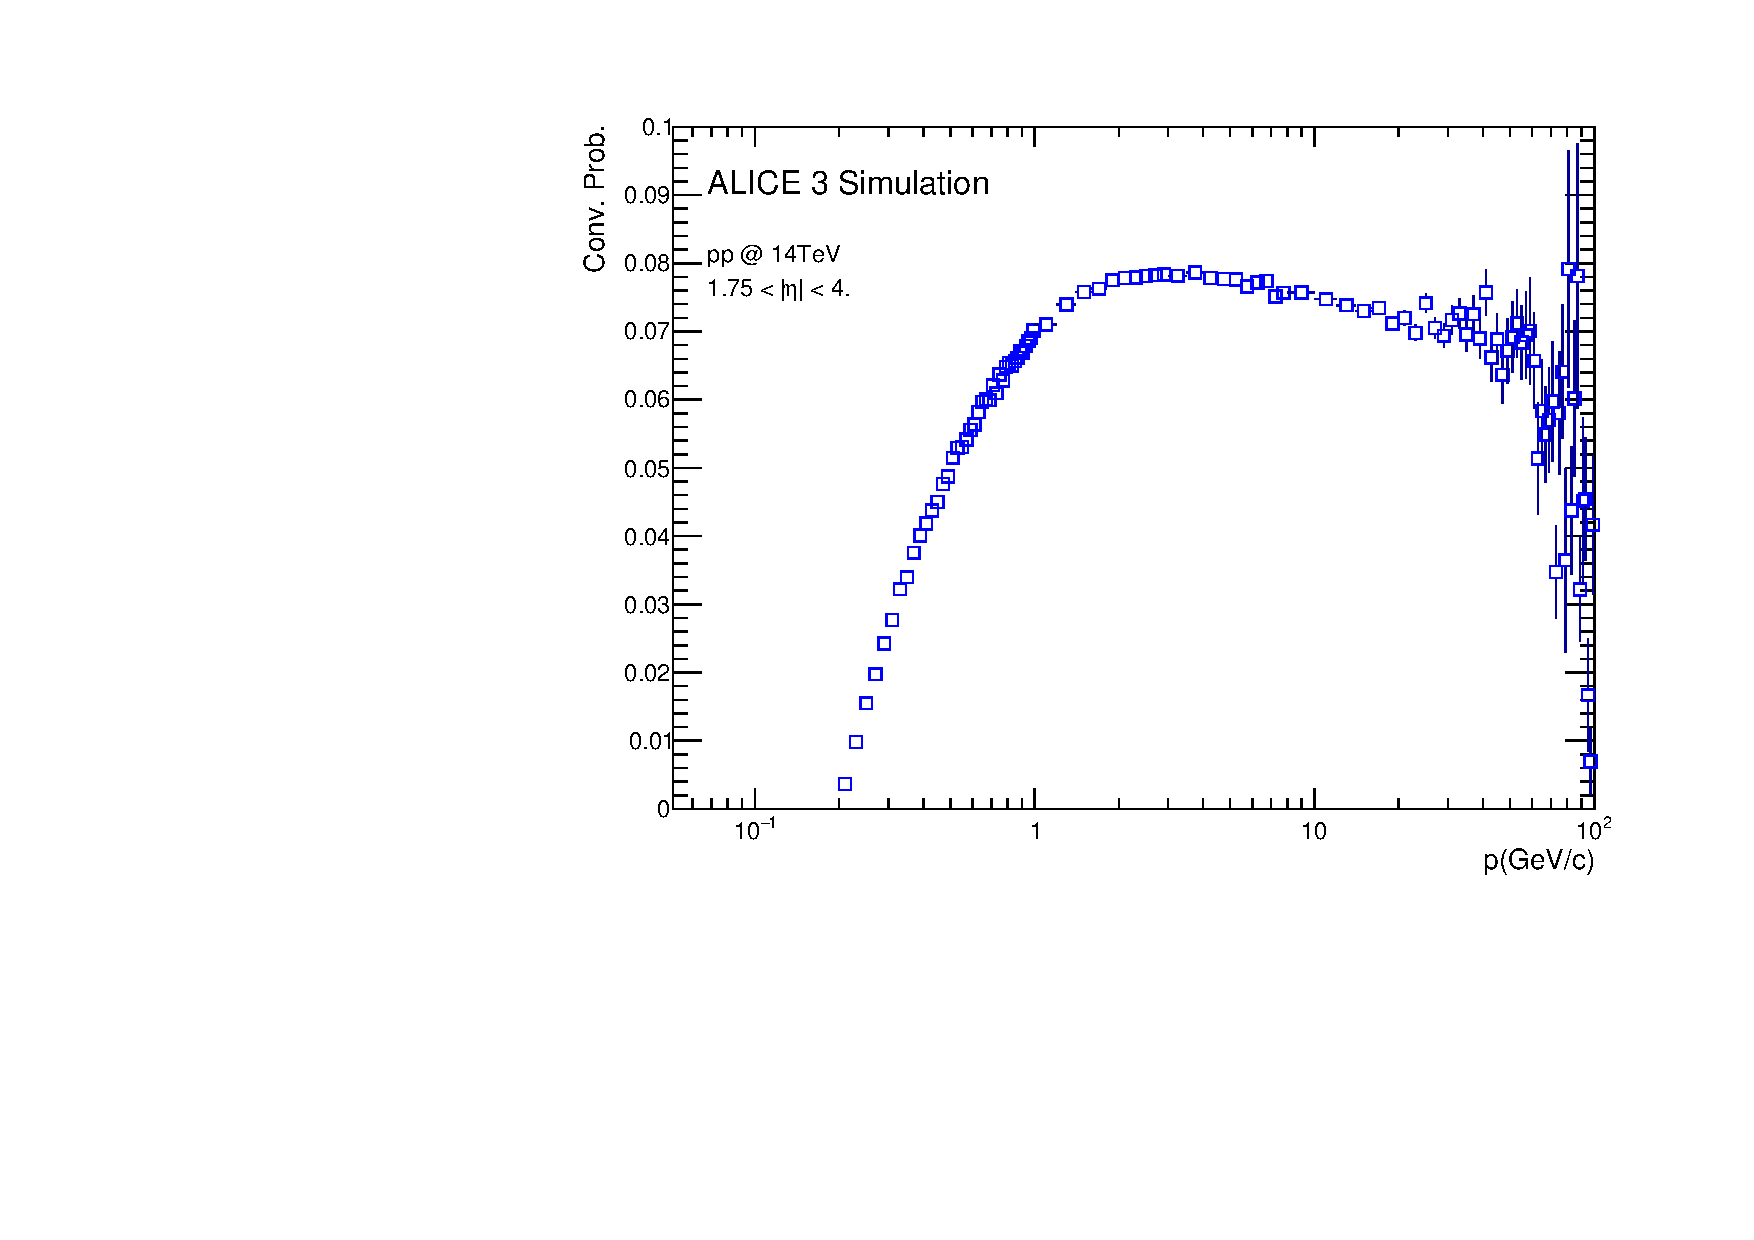
\includegraphics[width=0.4\textwidth]{/Users/marin/alice3/alice3Conversions/anaConv/files220103/PhotonConvProbF.pdf}
\end{frame}

\begin{frame}
\frametitle{Central Barrel: $\chi_{\rm C}$ $\rightarrow$ J/$\psi$ + $\gamma$} 

Delphes Simulation\\
\centering
\includegraphics[width=0.72\textwidth]{/Users/marin/alice3/chic/ChicMassPCM.pdf}

\end{frame}



\begin{frame}
\frametitle{PCM: Signal  estimation} 
\centering
\includegraphics[width=0.85\textwidth]{/Users/marin/alice3/chic/plots/fit_signal_chic_PCM.pdf}\\
%\includegraphics[width=0.48\textwidth]{/Users/marin/alice3/chic/plots/fit_bkg_chic_PCM.pdf}
\end{frame}

\begin{frame}
\frametitle{PCM: Background estimation} 
\centering
%\includegraphics[width=0.48\textwidth]{/Users/marin/alice3/chic/plots/fit_signal_chic_PCM.pdf}\\
\includegraphics[width=0.85\textwidth]{/Users/marin/alice3/chic/plots/fit_bkg_chic_PCM.pdf}
\end{frame}






\begin{frame}
\frametitle{Reconstruction efficiency: PCM and ECAL} 
\includegraphics[width=0.48\textwidth]{/Users/marin/alice3/chic/plots/Efficiency_chic_PCM.pdf}
\includegraphics[width=0.48\textwidth]{/Users/marin/alice3/chic/plots/Efficiency_chic_ECAL.pdf}

\end{frame}


\begin{frame}
\frametitle{Background per event: PCM and ECAL} 

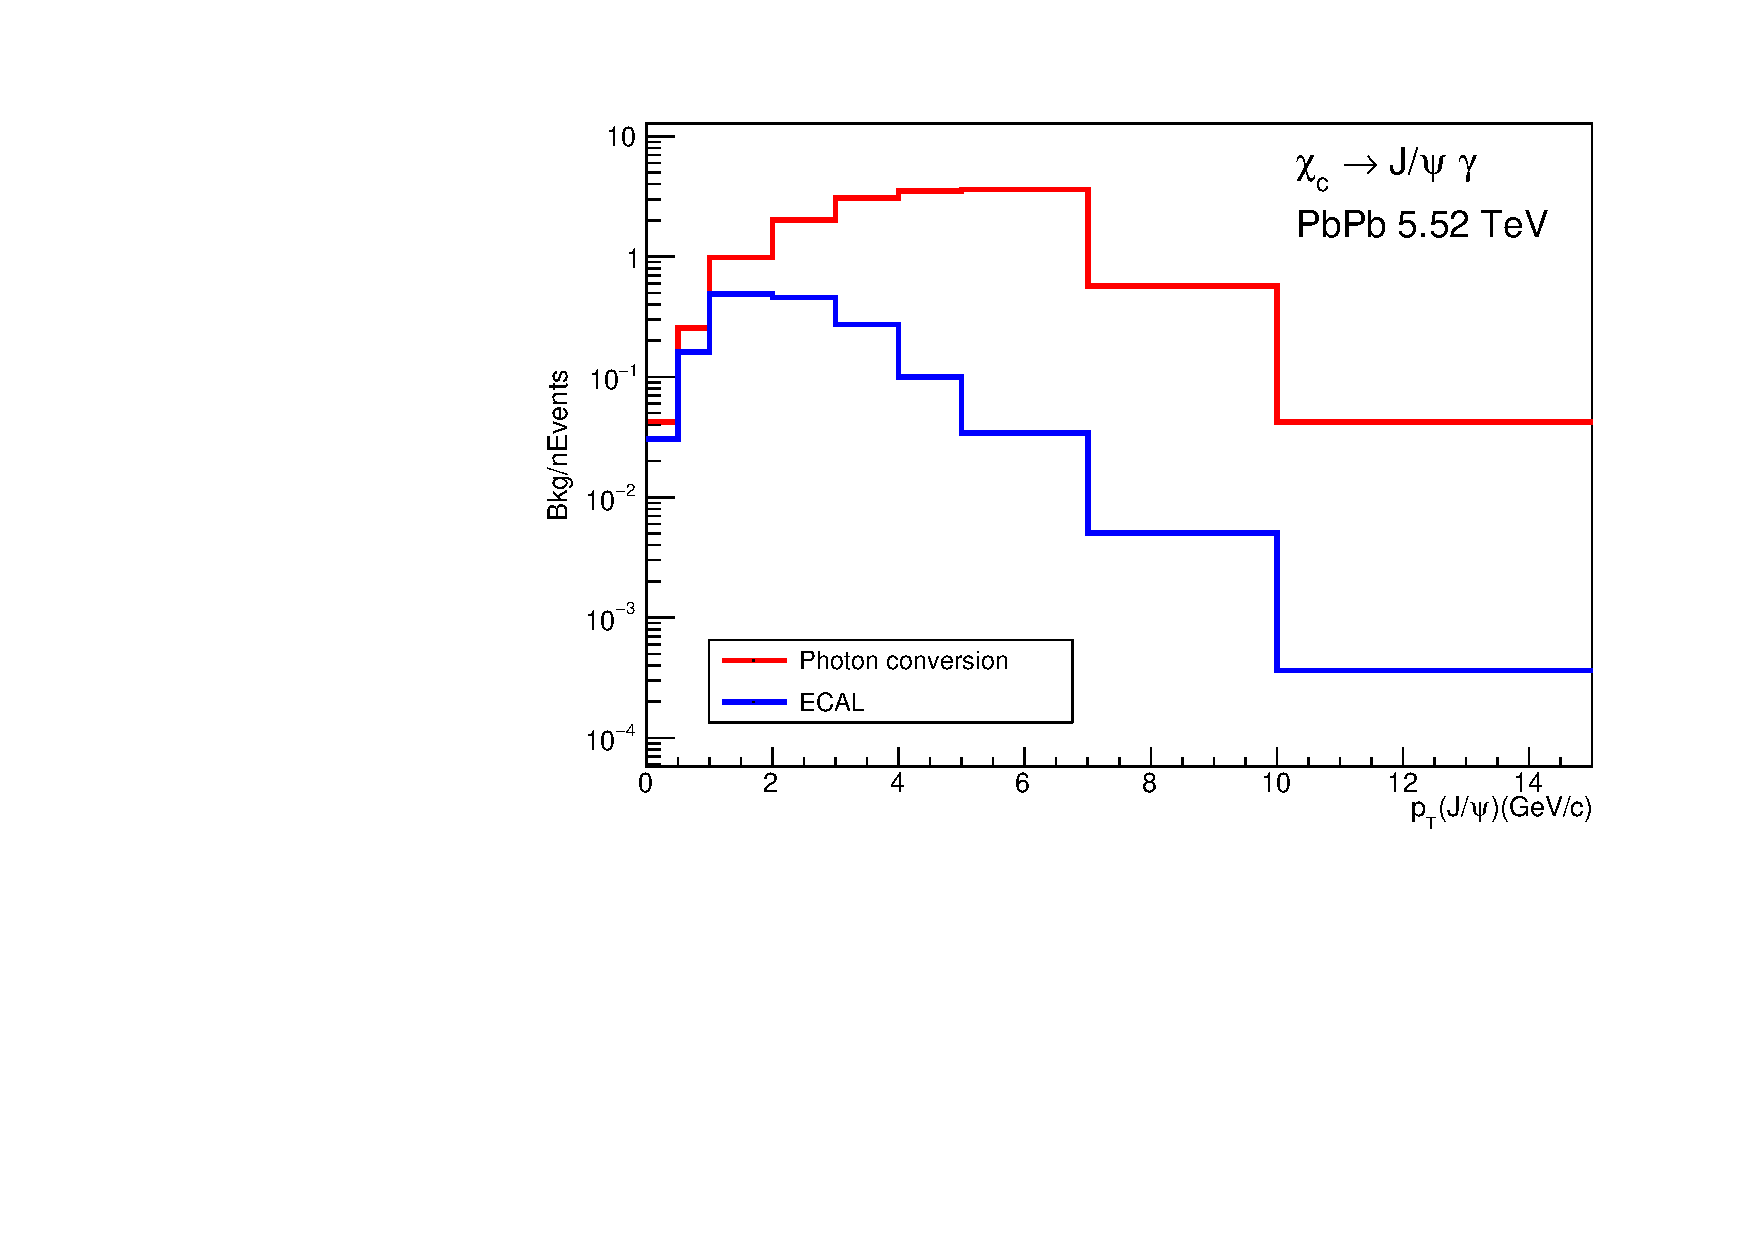
\includegraphics[width=0.48\textwidth]{/Users/marin/alice3/alice3Conversions//presentations/bkgPerEvent_chic_PbPb.pdf}
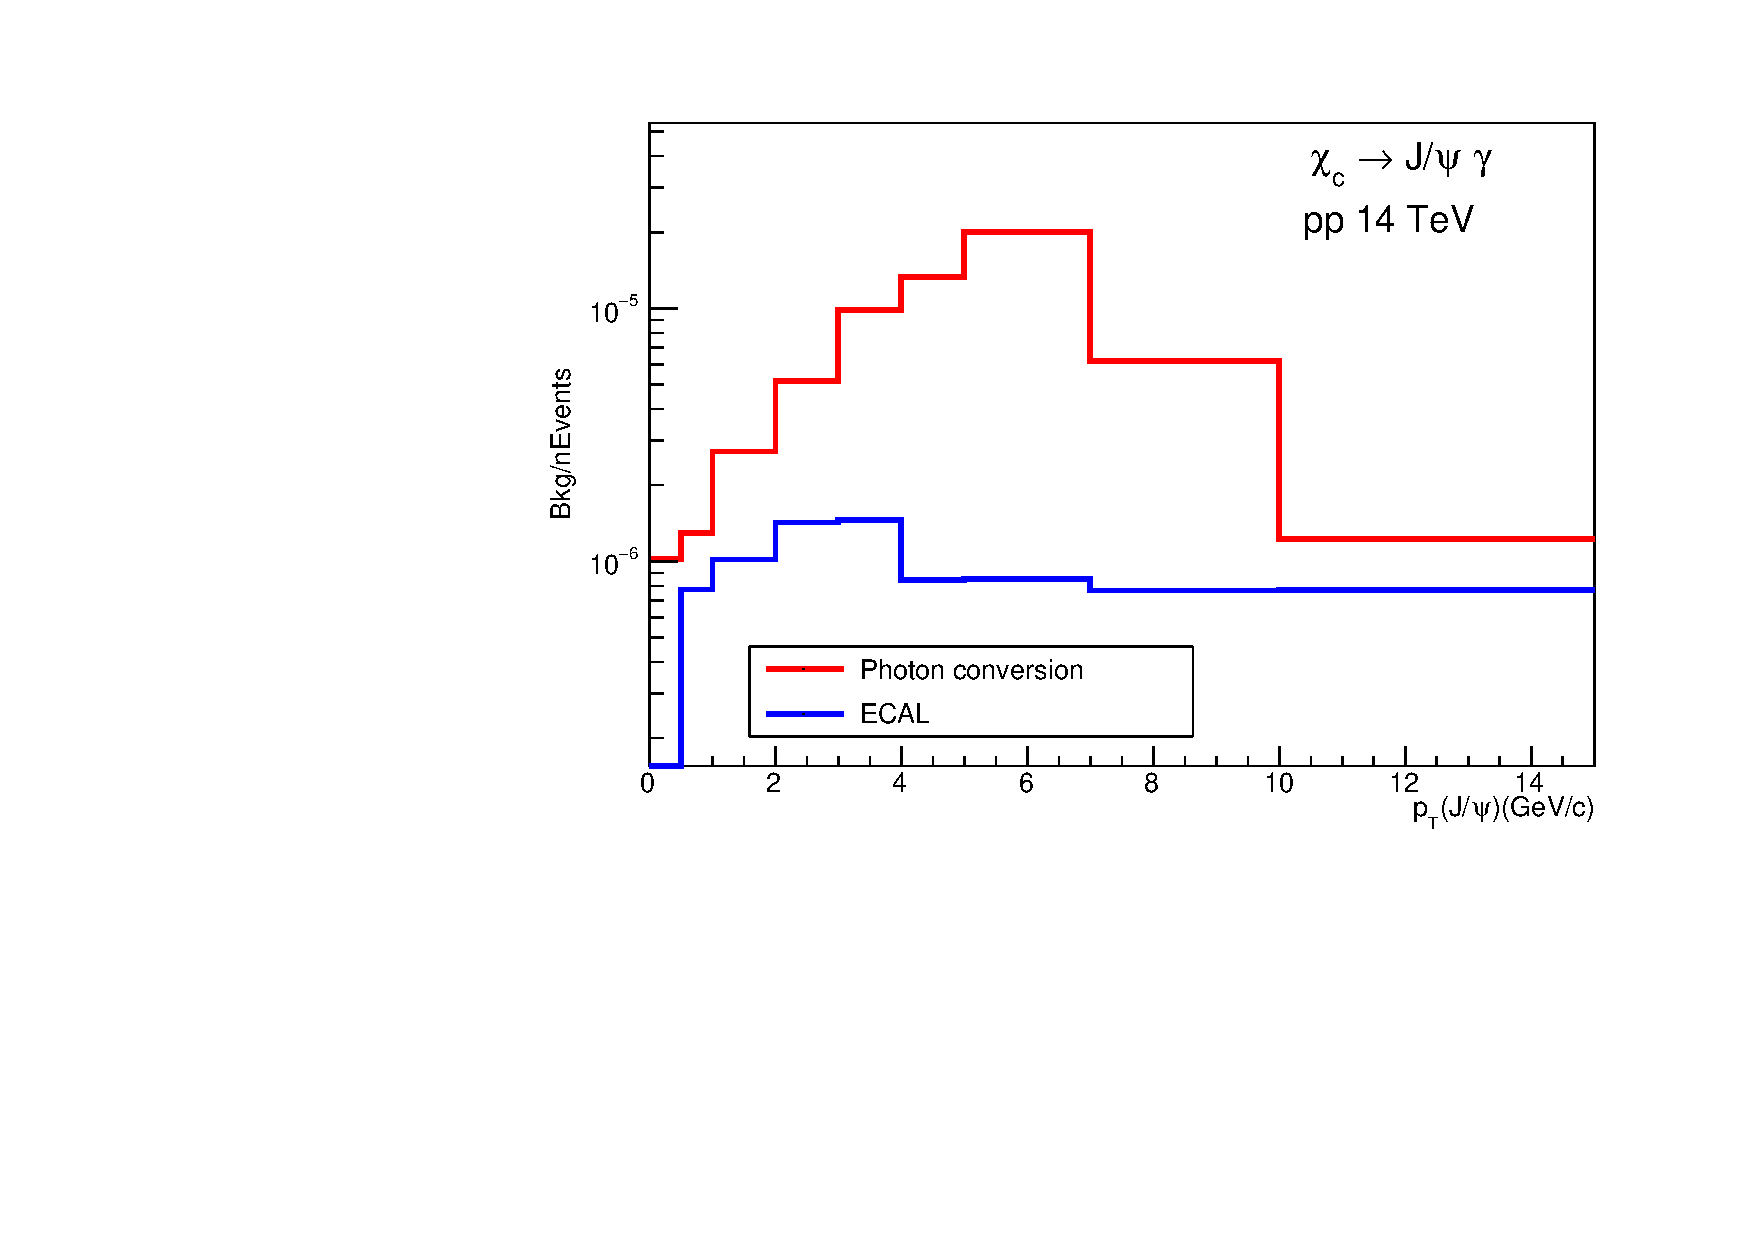
\includegraphics[width=0.48\textwidth]{/Users/marin/alice3/alice3Conversions//presentations/bkgPerEvent_chic_pp.pdf}
\end{frame}


\begin{frame}
\frametitle{Significance in pp: PCM and ECAL} 
\includegraphics[width=0.42\textwidth]{/Users/marin/alice3/chic/plots/Chi_c_PCM_pp14p0_absy1p44_results.pdf}
\includegraphics[width=0.42\textwidth]{/Users/marin/alice3/chic/plots/Chi_c_pp14p0_absy1p44_results.pdf}

Significance calculated as sum of $\chi_{\rm C1}$ and $\chi_{\rm C2}$\\
Combination of ECAL and PCM measurements will improve the significance

\end{frame}

\begin{frame}
\frametitle{Significance in PbPb: PCM and ECAL} 
\includegraphics[width=0.42\textwidth]{/Users/marin/alice3/chic/plots/Chi_c_PCM_PbPb5p52_absy1p44_results.pdf}
\includegraphics[width=0.42\textwidth]{/Users/marin/alice3/chic/plots/Chi_c_PbPb5p52_absy1p44_results.pdf}

Significance calculated as sum of $\chi_{\rm C1}$ and $\chi_{\rm C2}$\\
\end{frame}

\end{document}

\begin{frame}
\frametitle{Significance in pp: PCM and ECAL} 
\includegraphics[width=0.32\textwidth]{/Users/marin/alice3/chic/plots/Chi_c_PbPb5p52_absy1p44_results.pdf}
\includegraphics[width=0.32\textwidth]{/Users/marin/alice3/chic/plots/Chi_c_pp14p0_absy1p44_results.pdf}
\includegraphics[width=0.32\textwidth]{/Users/marin/alice3/chic/plots/Chi_c_PCM_pp14p0_absy1p44_results.pdf}
\includegraphics[width=0.32\textwidth]{/Users/marin/alice3/chic/plots/Chi_c_PCM_PbPb5p52_absy1p44_results.pdf}
\end{frame}




